\section{Alta, baja y modificación de datos (ABMs)}
En esta sección explicamos como realizar el alta, baja y modificación de datos del sistema, es decir, síntomas, discriminantes y usuarios.

\subsection{Acceso al menú de configuración}
Para poder acceder al menú de configuración de datos el usuario actual debe tener el rol de administrador. En caso contrario dicho menú permanecerá oculto (ver figuras \ref{fig:menu_conf_visible} y \ref{fig:menu_conf_oculto}).

\begin{figure}
\centerline{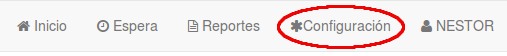
\includegraphics[width=0.7\textwidth]{menu_configuracion_visible.png}}
\caption{Menú de configuración visible}
\label{fig:menu_conf_visible}
\end{figure}

\begin{figure}
\centerline{
\includegraphics[width=0.7\textwidth]{menu_configuracion_oculto.png}}
\caption{Menú de configuración oculto}
\label{fig:menu_conf_oculto}
\end{figure}

\subsection{ABM de síntomas}
Para acceder a la pantalla de administración de síntomas nos dirigimos hacia ``Configuración'' y luego a ``Síntomas'' (ver figura \ref{fig:menu_sintomas}).
\begin{figure}
\centerline{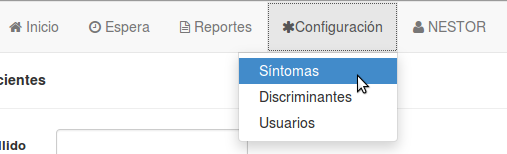
\includegraphics[width=0.7\textwidth]{menu_sintomas.png}}
\caption{Menú de síntomas}
\label{fig:menu_sintomas}
\end{figure}
Allí se nos muestra el listado de todos los síntomas cargados en el sistema (figura \ref{fig:listado_sintomas}).

\begin{figure}
\centerline{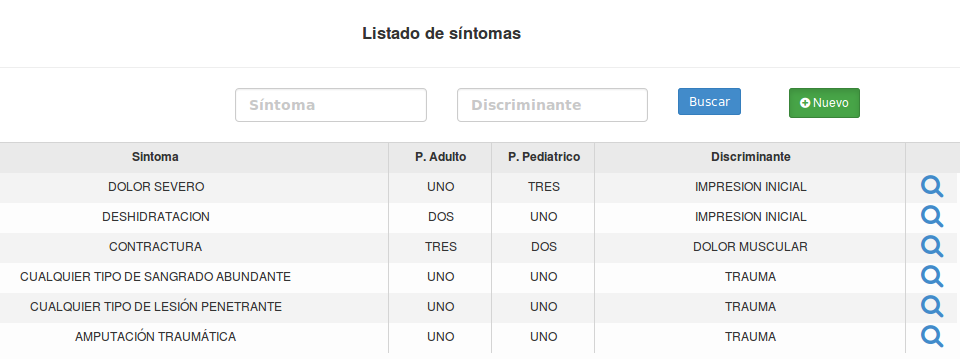
\includegraphics[width=1\textwidth]{listado_sintomas.png}}
\caption{Listado de síntomas}
\label{fig:listado_sintomas}
\end{figure}

\subsubsection{Alta de síntoma}
Para dar de alta un nuevo síntoma hacemos click en el botón ``Nuevo'', en la pantalla del listado de síntomas, que nos dirige a la pantalla del detalle del síntoma (figura \ref{fig:detalle_sintoma}).
\begin{figure}
\centerline{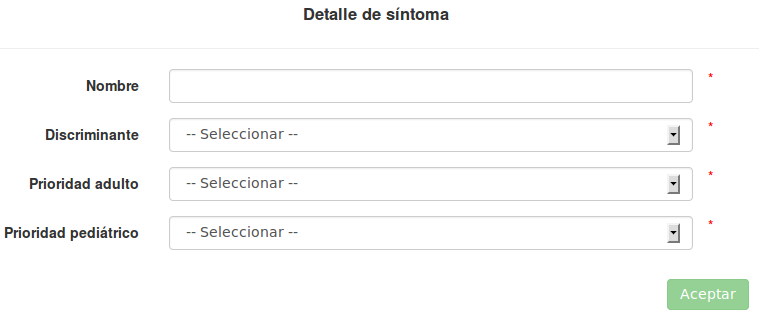
\includegraphics[width=1\textwidth]{detalle_sintoma.png}}
\caption{Detalle de síntoma}
\label{fig:detalle_sintoma}
\end{figure}
Allí debemos ingresar el nombre, el discriminante, la prioridad para adultos y la prioridad para pediátricos. Tener en cuenta que si el discriminante que deseamos no aparece en el listado desplegable entonces primero debemos ingresarlo en el ABM de discriminantes (Ver sección \ref{ABM_discriminantes}). Luego de llenar todos los campos, el botón ``Aceptar'' se desbloquea y si le hacemos click aparece un mensaje que confirma que el síntoma fue ingresado con éxito (figura \ref{fig:sintoma_cargado_con_exito}).
\begin{figure}
\centerline{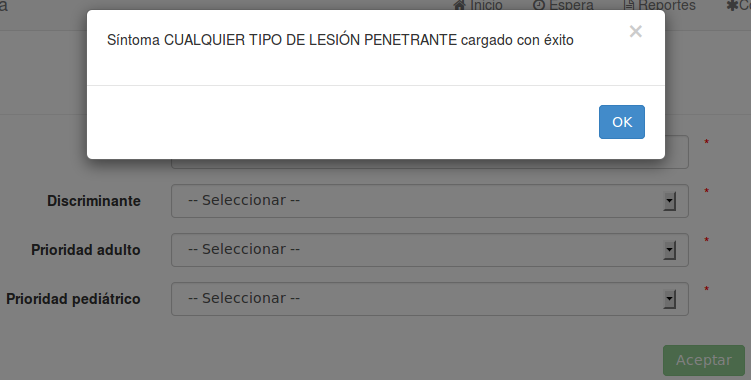
\includegraphics[width=1\textwidth]{sintoma_cargado_con_exito.png}}
\caption{Mensaje de síntoma cargado con éxito}
\label{fig:sintoma_cargado_con_exito}
\end{figure}

\subsubsection{Modificación de síntoma}
Para modificar un síntoma que hayamos dado de alta con anterioridad debemos seleccionarlo del listado de síntomas. Para facilitar la búsqueda del mismo podemos filtrar el listado llenando los campos de ``Síntoma'' y/o ``Discriminante''\footnote{El filtrado de los listados de síntomas, discriminantes y usuarios funciona de la misma manera. Por lo tanto en este manual sólo se explicará el filtrado del listado de síntomas.}. No hace falta que ingresemos la palabra entera. Es suficiente con ingresar las primeras letras. Tampoco se distinguen mayúsculas y minúsculas. Luego de ingresar el valor deseado hacemos click en el botón ``Buscar'' y si encontramos el síntoma buscado hacemos click en el botón ``Ver detalle''(ver figura \ref{fig:sintomas_filtro}) 
\begin{figure}
\centerline{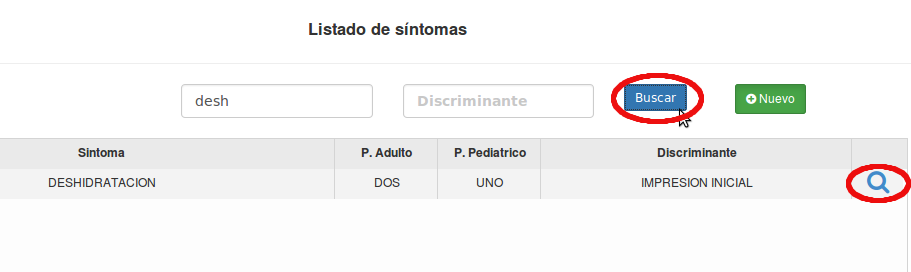
\includegraphics[width=1\textwidth]{sintomas_listado_buscar.png}}
\caption{Listado de síntomas filtrado. Aparecen los botones ``Buscar'' y ``Ver detalle'' señalados en rojo}
\label{fig:sintomas_filtro}
\end{figure}
que nos lleva a la pantalla de ``Detalle de síntoma'' con todos los campos cargados. Allí podemos modificar los valores que deseemos y al apretar ``Aceptar'' aparece el mensaje de confirmación de síntoma actualizado con éxito (figura \ref{fig:sintoma_actualizado_con_exito}).
\begin{figure}
\centerline{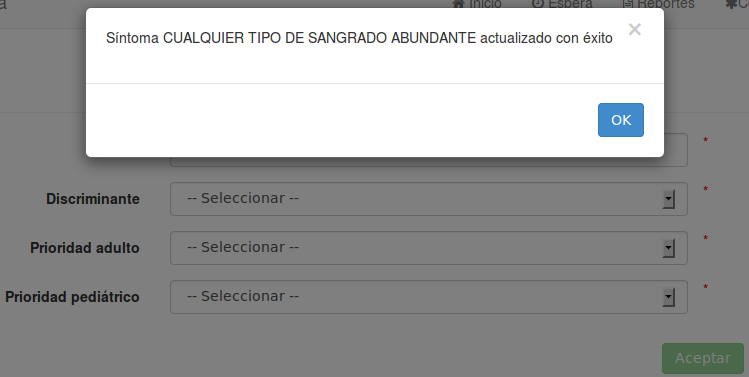
\includegraphics[width=1\textwidth]{sintoma_actualizado_con_exito.png}}
\caption{Mensaje de confirmación de síntoma actualizado con éxito}
\label{fig:sintoma_actualizado_con_exito}
\end{figure}

\subsubsection{Baja de síntoma}
Una vez creados, los síntomas no se pueden eliminar. Solo se pueden modificar como explicamos en la sección anterior. Lo mismo sucede con los discriminantes de síntomas.

\subsection{ABM de discriminantes de síntomas}\label{ABM_discriminantes}
Para acceder a la pantalla de administración de discriminantes de síntomas nos dirigimos hacia ``Configuración'' y luego a ``Discriminantes'' (ver figura \ref{fig:menu_discriminantes}).
\begin{figure}
\centerline{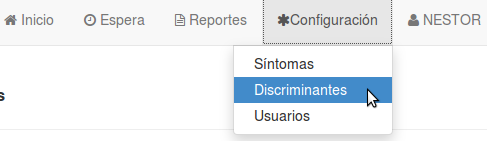
\includegraphics[width=0.7\textwidth]{menu_discriminantes.png}}
\caption{Menú de discriminantes de síntomas}
\label{fig:menu_discriminantes}
\end{figure}
Allí se nos muestra el listado de todos los discriminantes de síntomas cargados en el sistema (figura \ref{fig:listado_discriminantes}).
\begin{figure}
\centerline{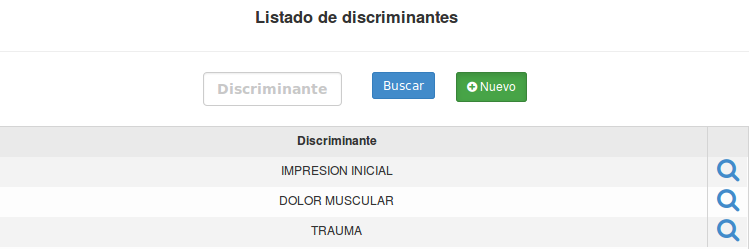
\includegraphics[width=1\textwidth]{listado_discriminantes.png}}
\caption{Listado de discriminantes}
\label{fig:listado_discriminantes}
\end{figure}




